% Created 2016-03-31 Thu 11:17
\documentclass{article}
\usepackage[utf8]{inputenc}
\usepackage[T1]{fontenc}
\usepackage{fixltx2e}
\usepackage{graphicx}
\usepackage{longtable}
\usepackage{float}
\usepackage{wrapfig}
\usepackage{rotating}
\usepackage[normalem]{ulem}
\usepackage{amsmath}
\usepackage{textcomp}
\usepackage{marvosym}
\usepackage{wasysym}
\usepackage{amssymb}
\usepackage{hyperref}
\tolerance=1000
\usepackage{minted}
\usepackage{listingsutf8}
\usepackage[bottom]{footmisc} %% to keep entire footers on one page
\usepackage[]{graphicx}
\usepackage[]{minted}
\usepackage[margin=1in]{geometry}
\usepackage{comment}
\usepackage[linesnumbered,ruled,lined,shortend]{algorithm2e}
\usepackage[space]{grffile}
\usepackage[bottom]{footmisc} %% to keep entire footers on one page
\usepackage[]{graphicx}
\usepackage[]{minted}
\usepackage[margin=1in]{geometry}
\usepackage{comment}
\usepackage[linesnumbered,ruled,lined,shortend]{algorithm2e}
\usepackage[space]{grffile}
\usepackage[bottom]{footmisc} %% to keep entire footers on one page
\usepackage[]{graphicx}
\usepackage[]{minted}
\usepackage[margin=1in]{geometry}
\usepackage{comment}
\usepackage[linesnumbered,ruled,lined,shortend]{algorithm2e}
\usepackage[space]{grffile}
\setcounter{secnumdepth}{4}
\author{Nicholas Mitchell}
\date{\today}
\title{6\_Appendices}
\hypersetup{
  pdfkeywords={},
  pdfsubject={},
  pdfcreator={Emacs 24.5.1 (Org mode 8.2.10)}}
\begin{document}

\maketitle
\tableofcontents



\section{Appendices}
\label{sec-1}



\subsection{Appendix 1 - Flowcharts \label{flowcharts}}
\label{sec-1-1}


\subsubsection{Flowchart 1 - Twitter mining \label{flowchart-twitter-mining}}
\label{sec-1-1-1}

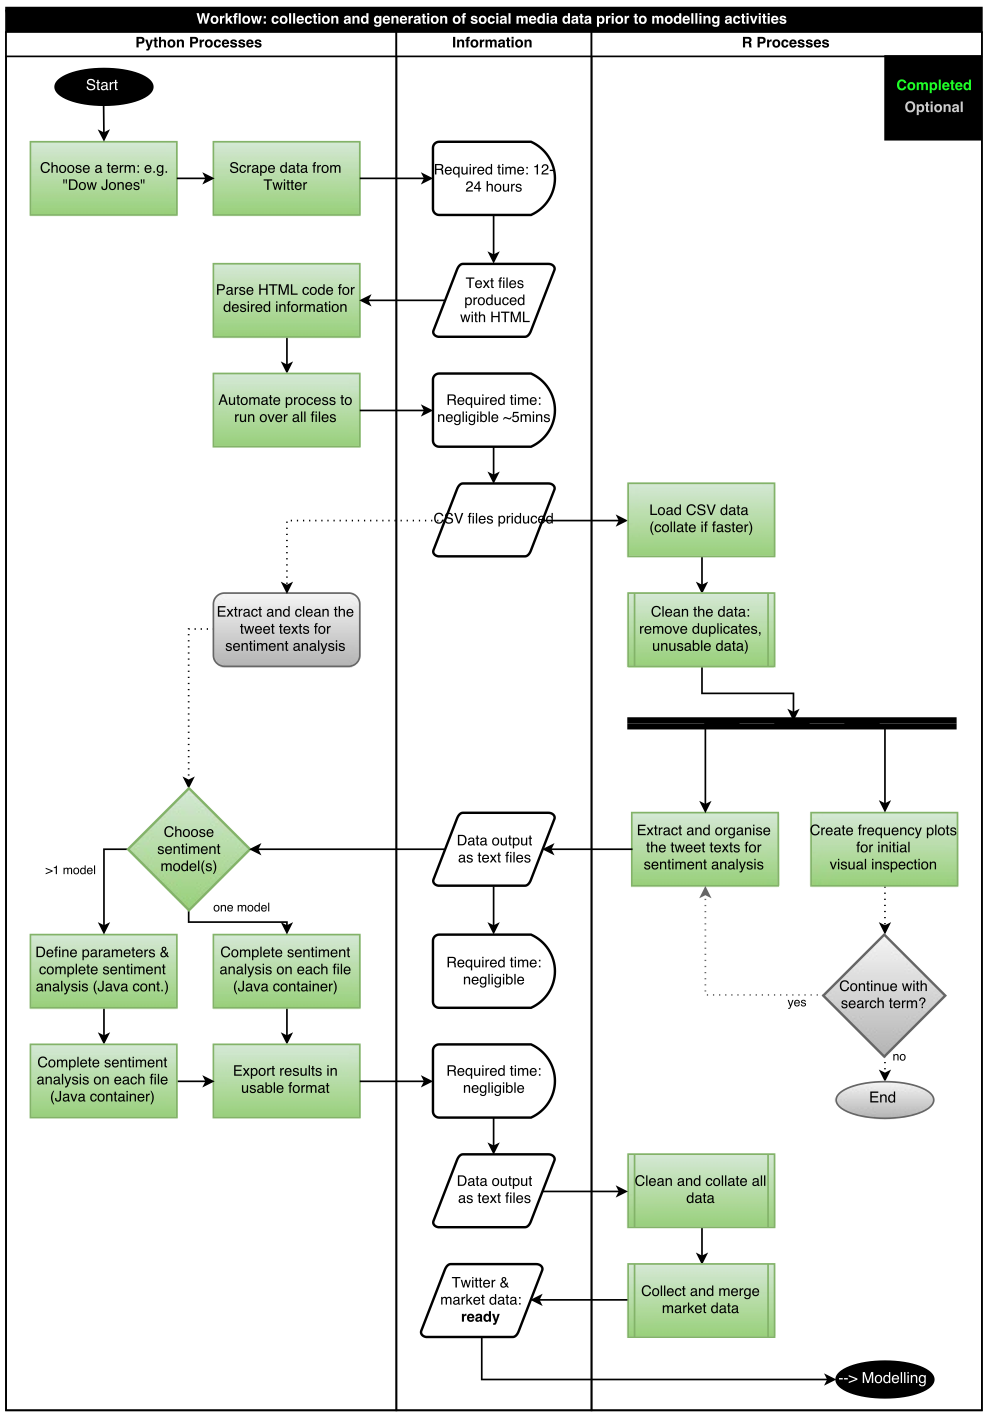
\includegraphics[width=14.5cm]{/Volumes/Mac OS Drive/Thesis/Source Code/Reporting/nwm_Report/images/workflow_scraping.png}


\subsubsection{Flowchart 2.a - Data preparation \label{flowchart-mod}}
\label{sec-1-1-2}

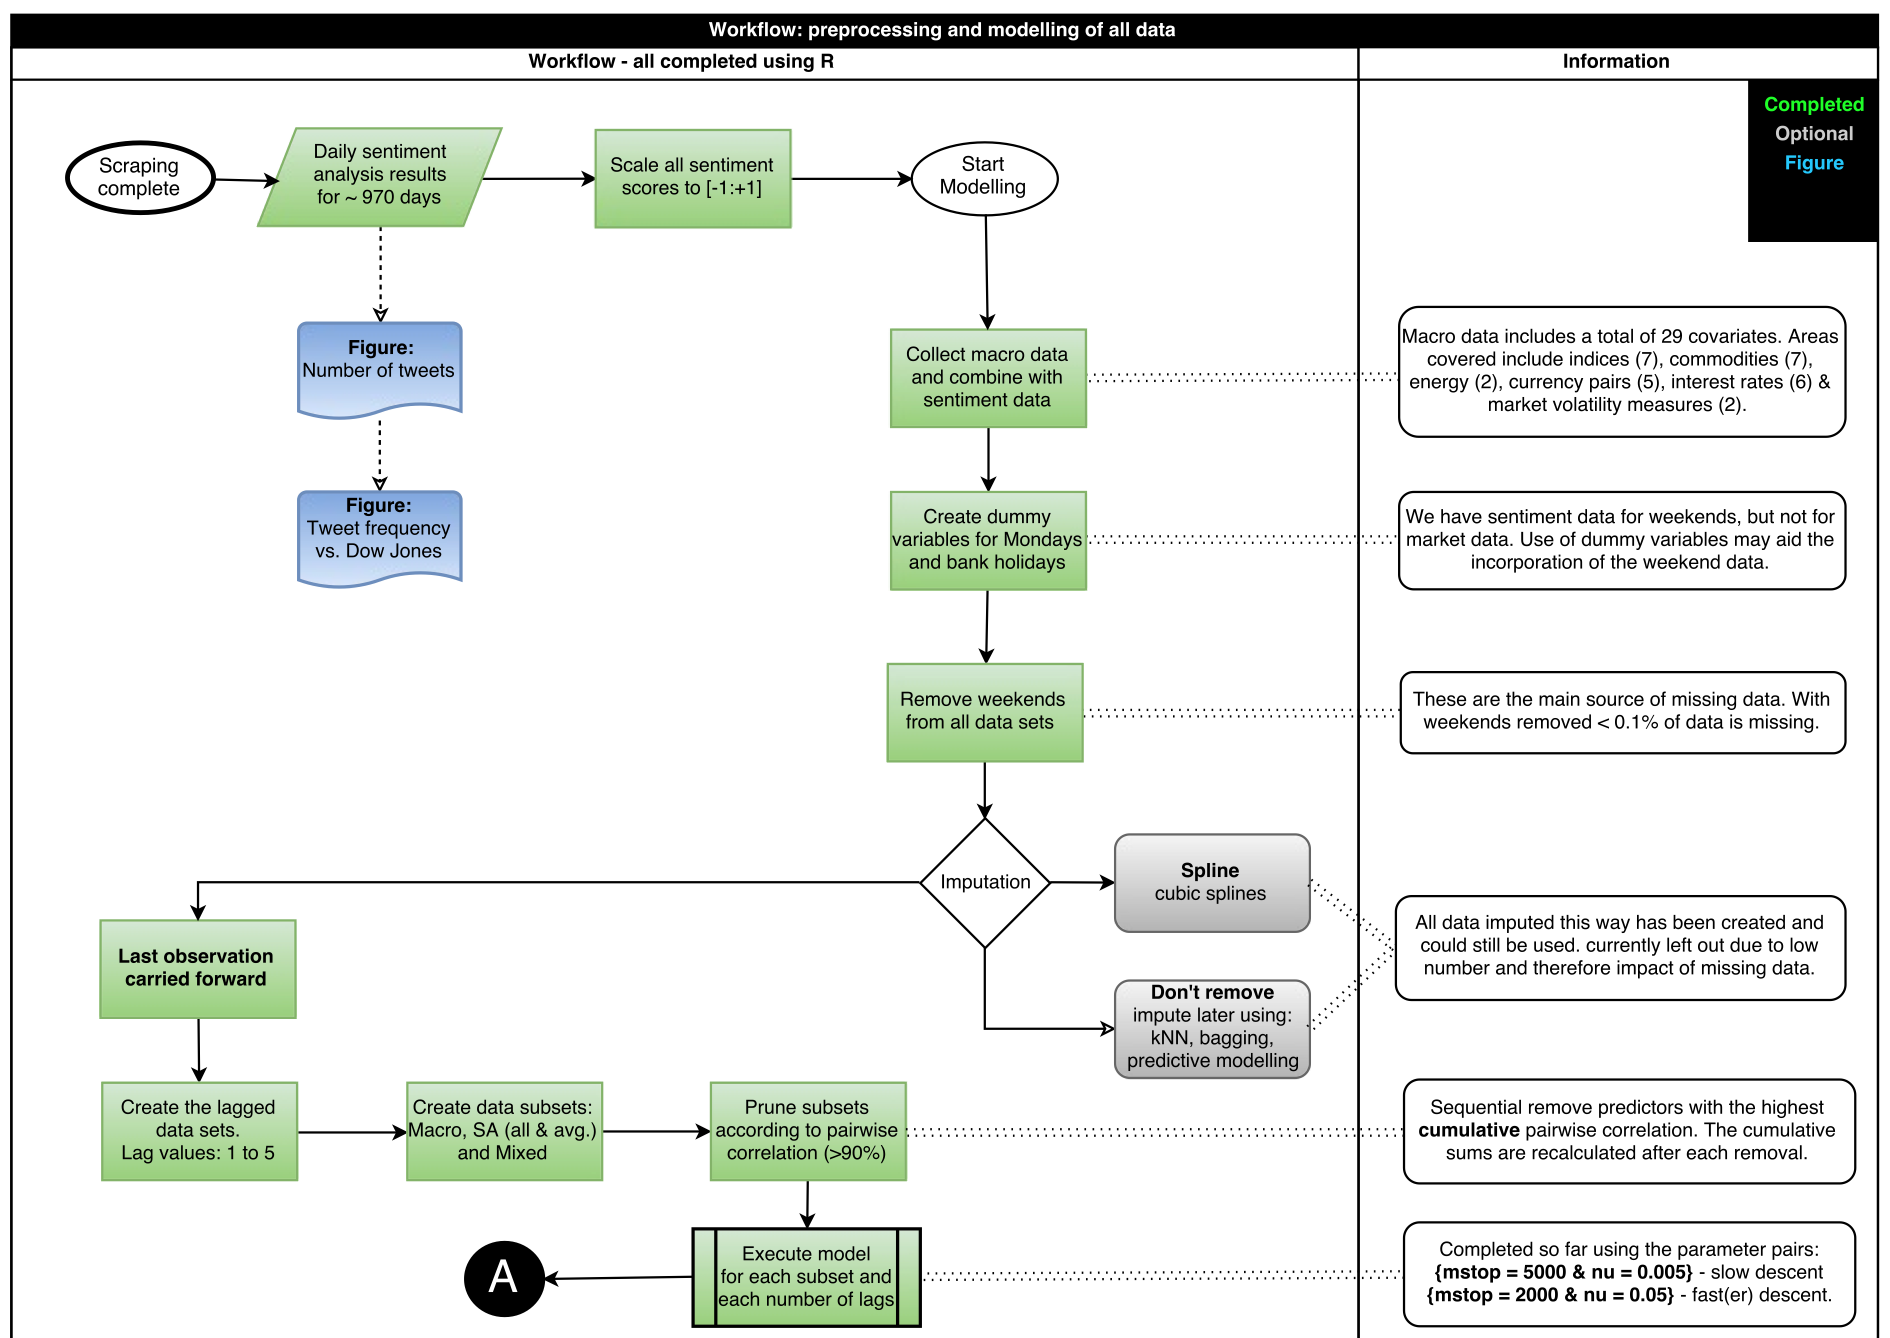
\includegraphics[angle=90,width=15.5cm]{/Volumes/Mac OS Drive/Thesis/Source Code/Reporting/nwm_Report/images/workflow_modelling_1.png}


\subsubsection{Flowchart 2.b - Modelling}
\label{sec-1-1-3}
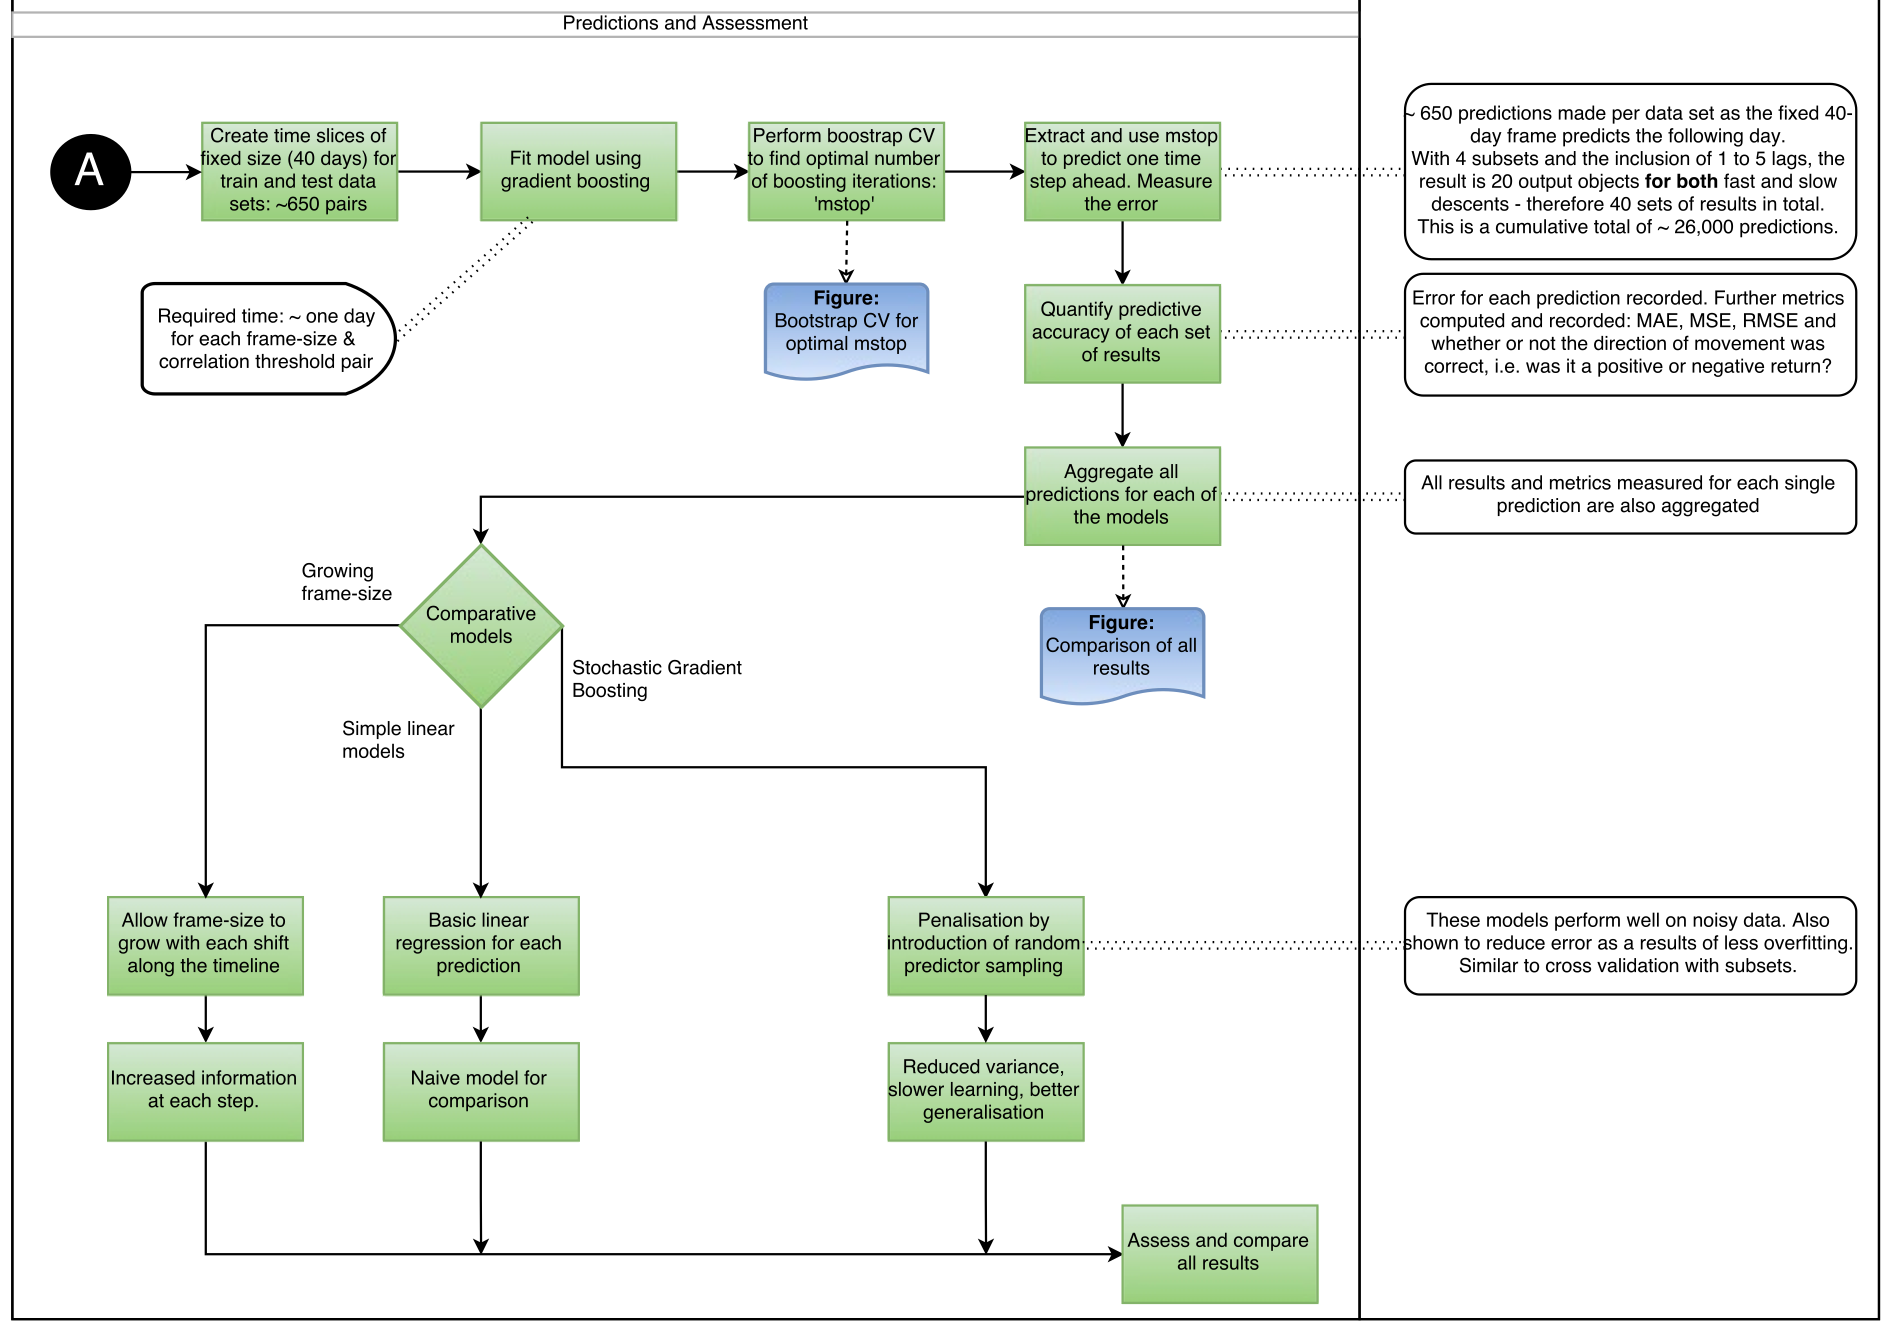
\includegraphics[angle=90,width=15.5cm]{/Volumes/Mac OS Drive/Thesis/Source Code/Reporting/nwm_Report/images/workflow_modelling_2.png}

\pagebreak

\pagebreak


\subsection{Appendix 2 - Public holidays \label{pub-holidays}}
\label{sec-1-2}


\subsubsection{Remark: Nikkei 225}
\label{sec-1-2-1}

An additional feature of the data sourced from \href{http://markets.on.nytimes.com/research/markets/holidays/holidays.asp?display\%3Dmarket&timeOffset\%3D-1&exchange\%3DTYO}{Japan} should be mentioned. The Nikkei 225 stock index data was used, which had a missing data point for the very first day of the timeline used, 14$^{\text{th}}$ January 2013. In order to perform the selected method of imputation - last observation carried forward (LOCF) - it was therefore necessary to source the data from the most closely preceding trading day, in order to impute Jan\}


\subsubsection{North America}
\label{sec-1-2-2}

Table \ref{tab:public-holidays} summarises public holidays relevant to the timeline and so the data used in this study is presented. The public holidays listed give the dates, which were used a dummy variables in the modelling. The dummy variable took the value 1 for a public holiday and 0 for not a public holiday.

\begin{table}\
\centering
\begin{tabular}{llllllllll}
\hline
 &  &  &  &  &  &  &  &  & \\
 &  &  &  &  &  &  &  & Monday January 21 2013 & \\
 & \textbf{Martin Luther King Day:} &  &  &  &  &  &  & Monday January 20 2014 & \\
 &  &  &  &  &  &  &  & Monday January 19 2015 & \\
 &  &  &  &  &  &  &  &  & \\
\hline
 &  &  &  &  &  &  &  &  & \\
 &  &  &  &  &  &  &  & Monday February 18 2013 & \\
 & \textbf{Presidents' Day:} &  &  &  &  &  &  & Monday February 17 2014 & \\
 &  &  &  &  &  &  &  & Monday February 16 2015 & \\
 &  &  &  &  &  &  &  &  & \\
\hline
 &  &  &  &  &  &  &  &  & \\
 &  &  &  &  &  &  &  & Monday May 27 2013 & \\
 & \textbf{Memorial Day:} &  &  &  &  &  &  & Monday May 26 2014 & \\
 &  &  &  &  &  &  &  & Monday May 25 2015 & \\
 &  &  &  &  &  &  &  &  & \\
\hline
 &  &  &  &  &  &  &  &  & \\
 &  &  &  &  &  &  &  & Thursday July 4 2013 & \\
 & \textbf{Independence Day:} &  &  &  &  &  &  & Friday July 4 2014 & \\
 &  &  &  &  &  &  &  & Friday July 3 2015 & \\
 &  &  &  &  &  &  &  &  & \\
\hline
 &  &  &  &  &  &  &  &  & \\
 &  &  &  &  &  &  &  & Monday September 2 2013 & \\
 & \textbf{Labor Day:} &  &  &  &  &  &  & Monday September 1 2014 & \\
 &  &  &  &  &  &  &  & Monday September 7 2015 & \\
 &  &  &  &  &  &  &  &  & \\
\hline
 &  &  &  &  &  &  &  &  & \\
 & \textbf{Columbus Day:} &  &  &  &  &  &  & Monday October 14 2013 & \\
 &  &  &  &  &  &  &  &  & \\
\hline
 &  &  &  &  &  &  &  &  & \\
 & \textbf{Veterans' Day:} &  &  &  &  &  &  & Monday November 11 2013 & \\
 &  &  &  &  &  &  &  & Tuesday November 11 2014 & \\
 &  &  &  &  &  &  &  &  & \\
\hline
 &  &  &  &  &  &  &  &  & \\
 & \textbf{Thanksgiving Day:} &  &  &  &  &  &  & Thursday November 28 2013 & \\
 &  &  &  &  &  &  &  & Thursday November 27 2014 & \\
 &  &  &  &  &  &  &  &  & \\
\hline
 &  &  &  &  &  &  &  &  & \\
 & \textbf{Christmas Day:} &  &  &  &  &  &  & Wednesday December 25 2013 & \\
 &  &  &  &  &  &  &  & Thursday December 25 2014 & \\
 &  &  &  &  &  &  &  &  & \\
\hline
 &  &  &  &  &  &  &  &  & \\
 & \textbf{New Year's Day:} &  &  &  &  &  &  & Wednesday January 1 2014 & \\
 &  &  &  &  &  &  &  & Thursday January 1 2015 & \\
 &  &  &  &  &  &  &  &  & \\
\hline
 &  &  &  &  &  &  &  &  & \\
 & \textbf{Columbus Day:} &  &  &  &  &  &  & Monday October 13 2014 & \\
 &  &  &  &  &  &  &  &  & \\
\hline
\end{tabular}\caption{\label{tab:public-holidays}A summary of relevant public holidays in North America, included as a dummy variable for modelling.}

\end{table}

\pagebreak
% Emacs 24.5.1 (Org mode 8.2.10)
\end{document}